\section{Detail nabídky}

\label{nur:detail}

Existují 2 verze zobrazení detailu nabídky. A~to zobrazení spolu s~mapou a zobrazení na samostatné stránce.

\subsection{Zobrazení spolu s~mapou}
Tímto způsobem se zobrazují pouze nabídky, které jsou volné\footnote{Stav nabídky je \textit{Čeká na druhého uživatele}.}. V~mapě se zobrazuje čára mezi umístěním uživatele a umístěním nabídky. V~textové části pak základní informace o~nabídce a dále také informace o~uživateli. Stránka dále obsahuje tlačítko, které slouží k~projevení zájmu o~danou nabídku. V~případě, že již uživatel má nějaké zkušenosti s~tímto uživatelem, jsou zobrazeny jejich společné nabídky. Z~detailu nabídky se lze vrátit zpět na výpis nabídek pomocí tlačítka \textit{Zpět} (Back). Detail nabídky lze vidět na obrázku \ref{fig:tur:offer-detail-map}.

\begin{figure}[!h]
    \centering
    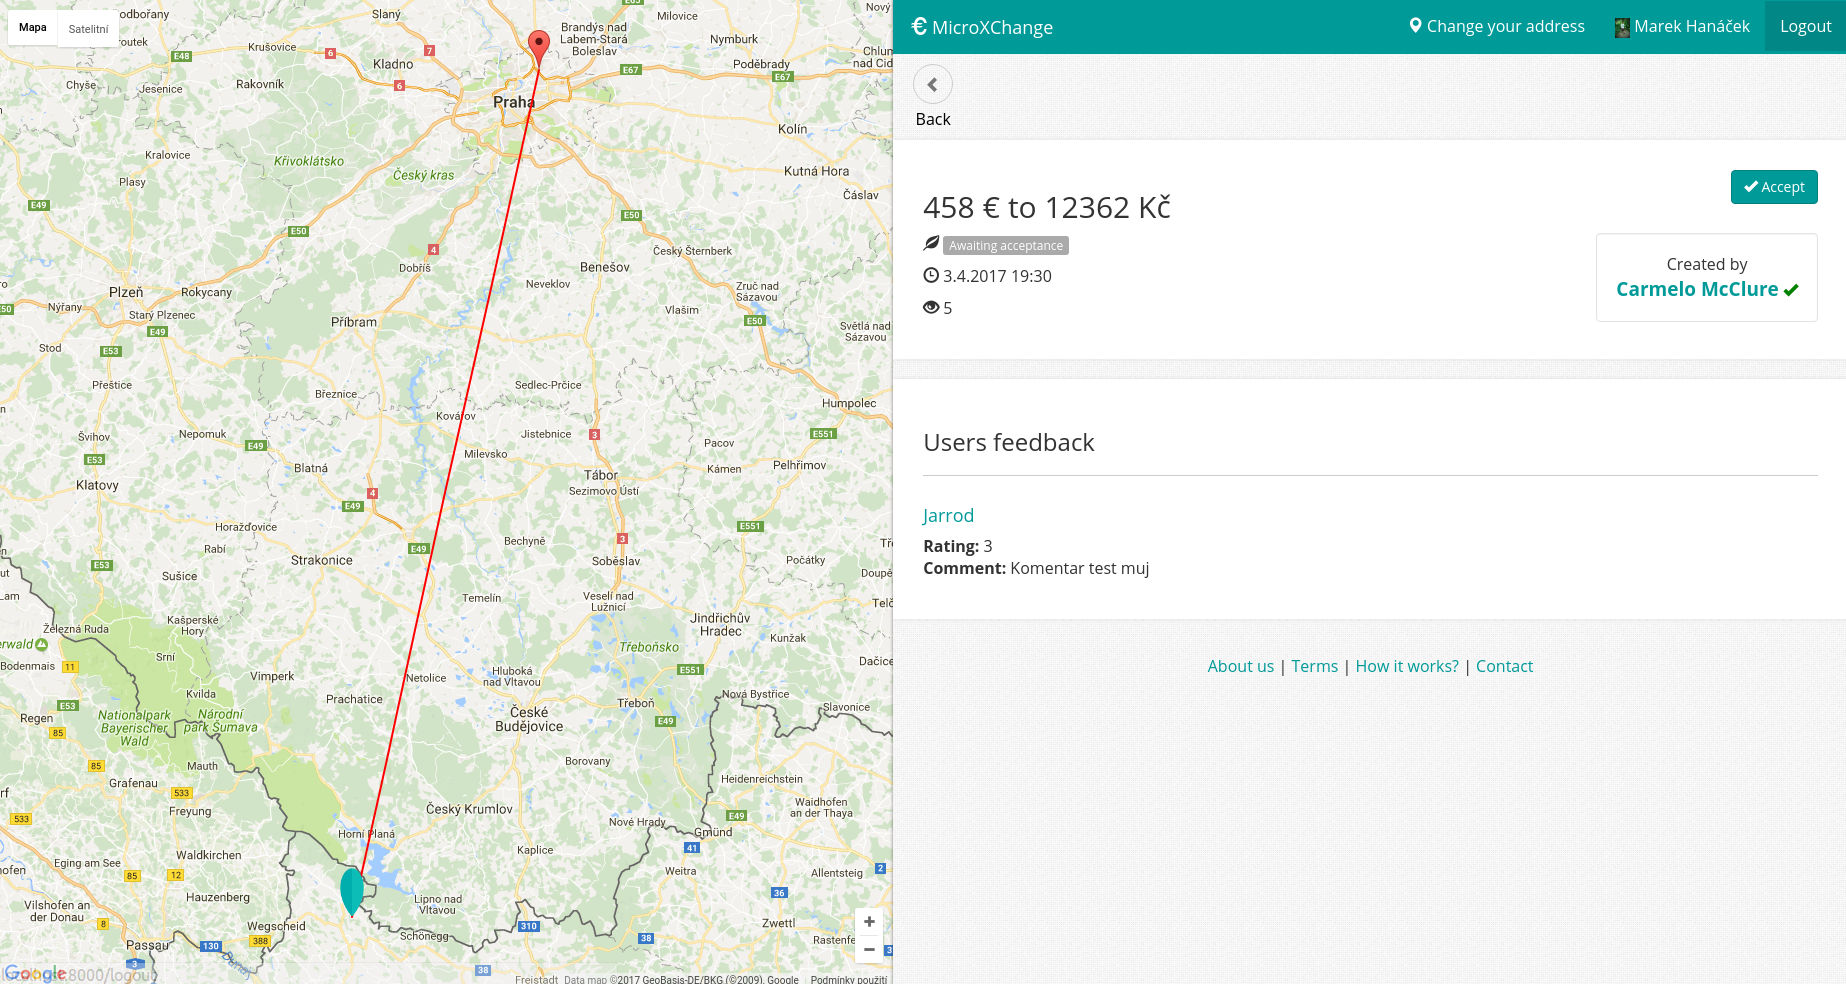
\includegraphics[width=1.0\textwidth]{media/tur/offer-detail-map.png}
    \caption{Detail nabídky s~mapou}
    \label{fig:tur:offer-detail-map}
\end{figure}

\subsection{Zobrazení na samostatné stránce}
Zobrazení je dostupné pouze v~případě, že uživatel je přiřazen k~nabídce. Toto zobrazení obsahuje totožné informace jako zobrazení s~mapou. Při rozvržení bez mapy však máme více prostoru a detail nabídky je tedy uspořádán jinak. Na toto zobrazení se uživatel dostane ze svého uživatelského profilu. Detail nabídky s~tímto rozvržením lze vidět na obrázku \ref{fig:tur:offer-detail-no-map} na straně \pageref{fig:tur:offer-detail-no-map}.

\begin{figure}[!h]
    \centering
    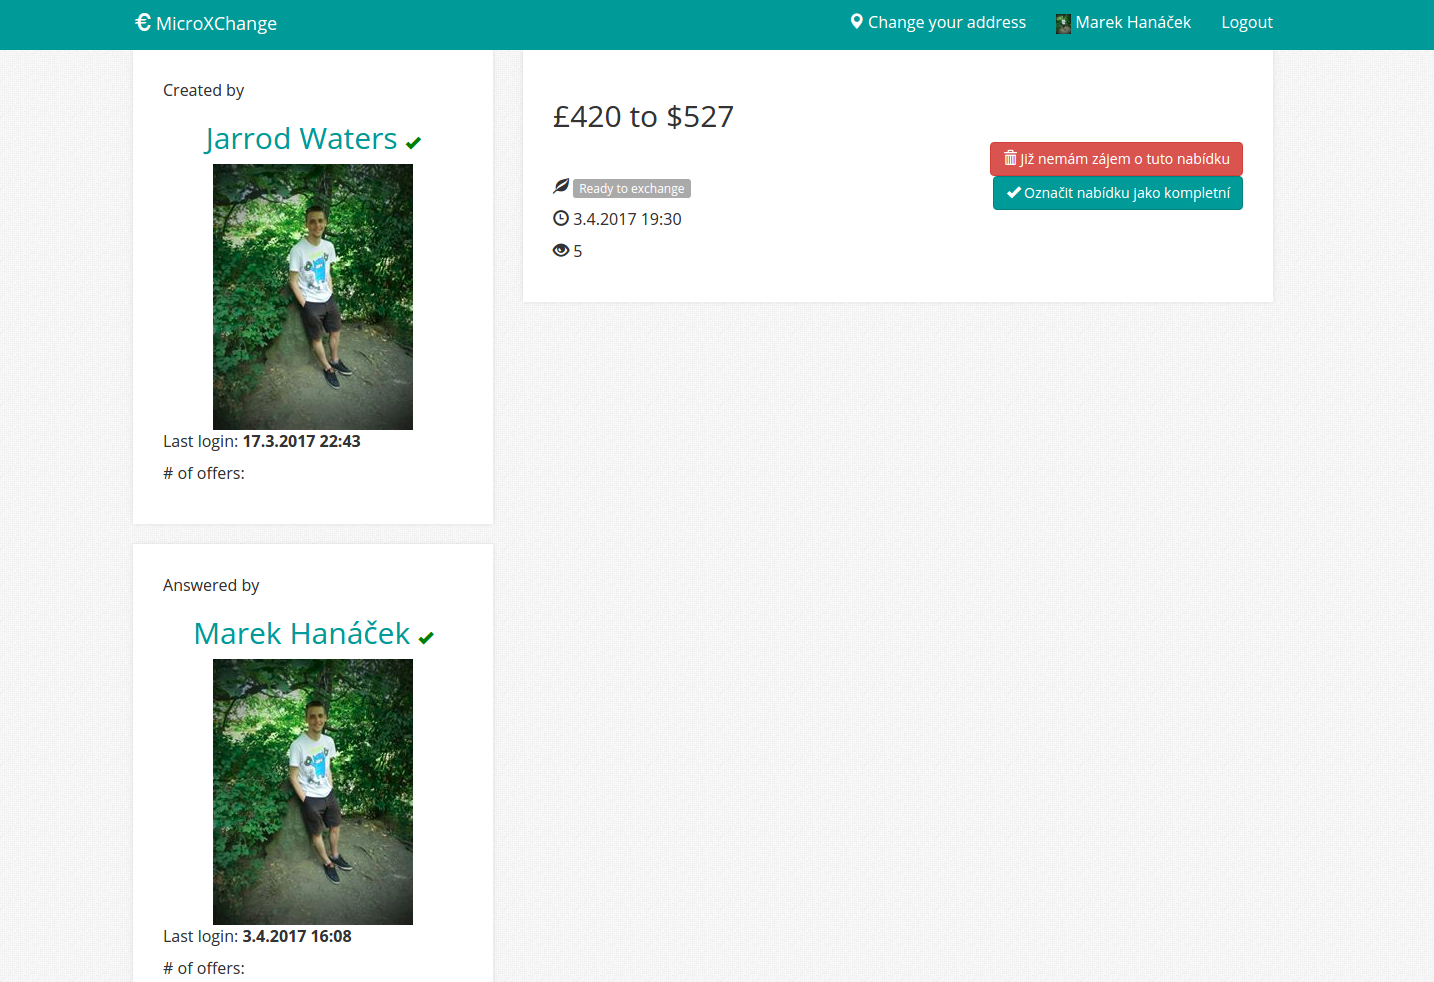
\includegraphics[width=1.0\textwidth]{media/tur/offer-detail-no-map.png}
    \caption{Detail nabídky bez mapy}
    \label{fig:tur:offer-detail-no-map}
\end{figure}